\documentclass[pdflatex,compress]{beamer}

%\usetheme[dark,framenumber,totalframenumber]{ElektroITK}
\usetheme[darktitle,framenumber,totalframenumber]{ElektroITK}
\usepackage{graphicx}
\usepackage{multicol}

\title{Data Communications}
\subtitle{Chapter 7 - Flow and Error Control}

\author{Mifta Nur Farid}

\begin{document}

\maketitle

\begin{frame}
	\frametitle{Data Link Control Protocols}
	\begin{itemize}
		\item Requirements and objectives for effective data communication between two directly connected transmitting-receiving stations:
		\begin{enumerate}
			\item Frame synchronization
			\item Flow control
			\item Error control
			\item Addressing
			\item Control and data
			\item Link management
		\end{enumerate}
	\end{itemize}
\end{frame}

\begin{frame}
	\frametitle{Flow Control}
	\begin{itemize}
		\item Technique for assuring that a transmitting entity does not over-whelm a receiving entity with data
		\item In the absence of flow control, the receiver’s buffer may fill up and overflow while it is processing old data
	\end{itemize}
\end{frame}

\begin{frame}
	\frametitle{Model of Frame Transmission}
	\begin{center}
		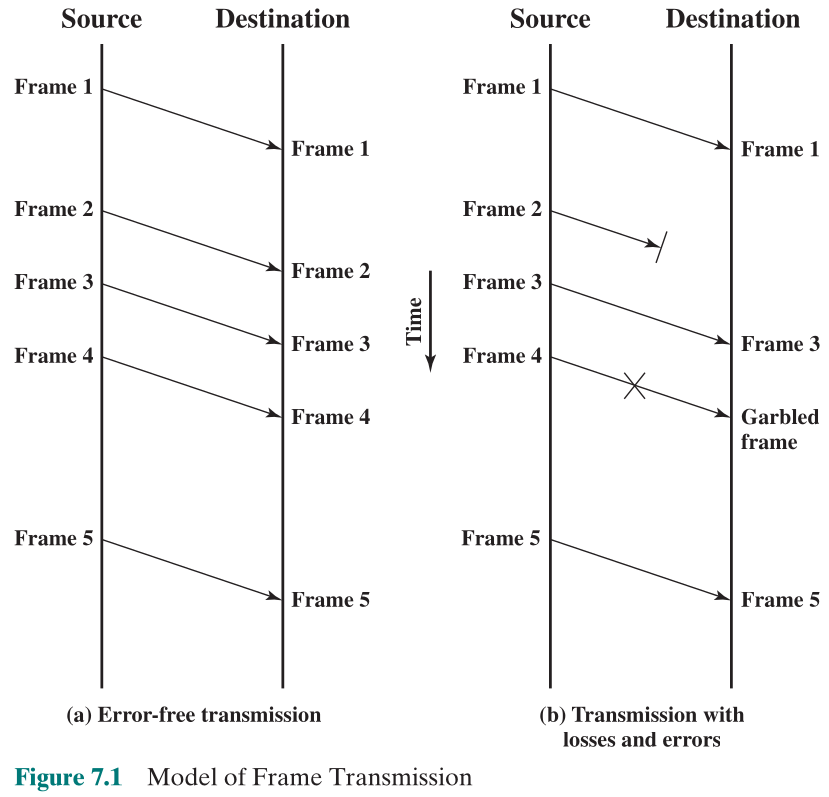
\includegraphics[width=0.6\linewidth]{img/img01}
	\end{center}
\end{frame}

\begin{frame}
	\frametitle{Stop-and-Wait Flow Control}
	\begin{itemize}
		\item Simplest form of flow control
		\begin{enumerate}
			\item Source transmits frame
			\item Destination receives frame and replies with acknowledgement (ACK)
			\item Source waits for ACK before sending next frame
			\item Destination can stop flow by not send ACK
		\end{enumerate}
	\end{itemize}
\end{frame}

\begin{frame}{Stop-and-Wait Flow Control}
	\begin{itemize}
		\item It is often the case that a source will break up a large block of data into smaller blocks and transmit the data in many frames
		\begin{itemize}
			\item The buffer size of the receiver may be limited
			\item The longer the transmission, the more likely that there will be an error, necessitating retransmission of the entire frame
			\item On a shared medium it is usually desirable not to permit one station to use the medium for an extended period, thus causing long delays at the other sending station
		\end{itemize}
	\end{itemize}
\end{frame}

\begin{frame}{Stop-and-Wait Link Utilization}
	\begin{center}
		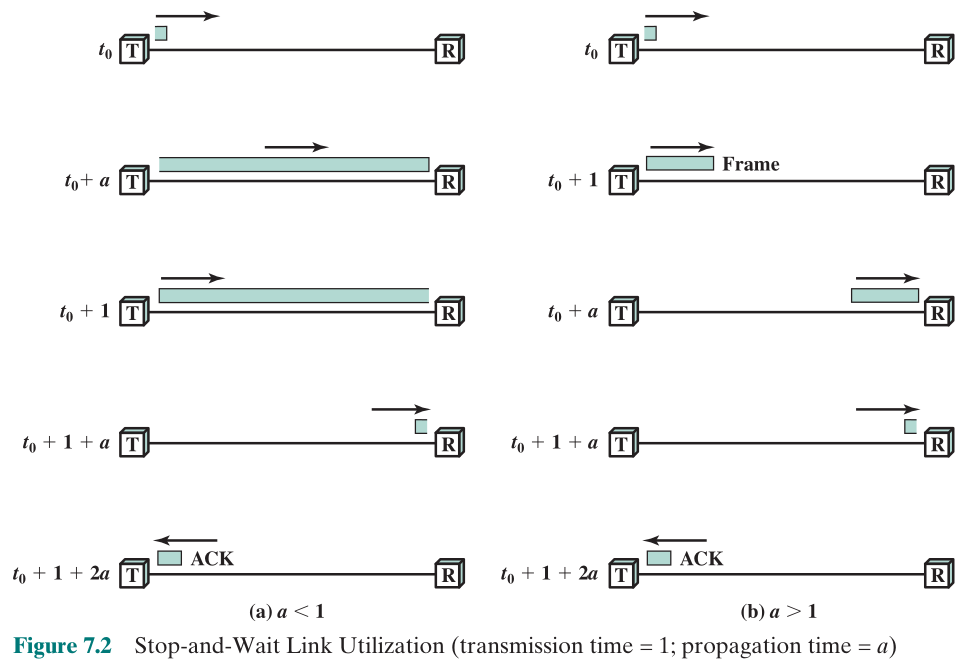
\includegraphics[width=0.9\linewidth]{img/img02}
	\end{center}
\end{frame}

\begin{frame}
	\frametitle{Sliding Windows Flow Control}
	\begin{itemize}
		\item Allows multiple numbered frames to be in transit
		\begin{itemize}
			\item Receiver has \textbf{buffer W} long
			\item Transmitter sends up to W frames without ACK
			\item \textbf{ACK includes number} of next frame expected
			\item \textbf{Sequence number} is bounded by \textbf{size of field (k)}
			\begin{itemize}
				\item Frames are numbered modulo $ 2^k $
				\item \textbf{Giving max window size of up to $ 2^k - 1 $}
			\end{itemize}
			\item Receiver can ACK frames without permitting further transmission (Receive Not Ready)
			\item Must send a normal acknowledge to resume
		\end{itemize}
		\item If have full-duplex link, can piggyback ACKs
	\end{itemize}
\end{frame}

\begin{frame}
	\frametitle{Sliding Window Diagram}
	\begin{flushright}
		3-bit seq, W = 7 frames
	\end{flushright}
	\begin{center}
		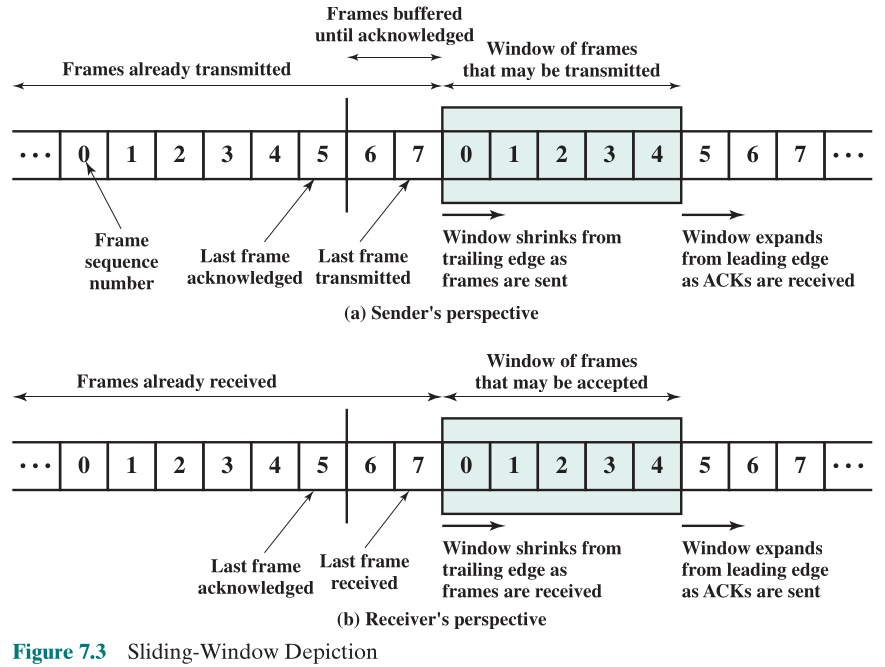
\includegraphics[width=0.8\linewidth]{img/img03}
	\end{center}
\end{frame}

\begin{frame}
	\frametitle{Sliding Window Example}
	\begin{center}
		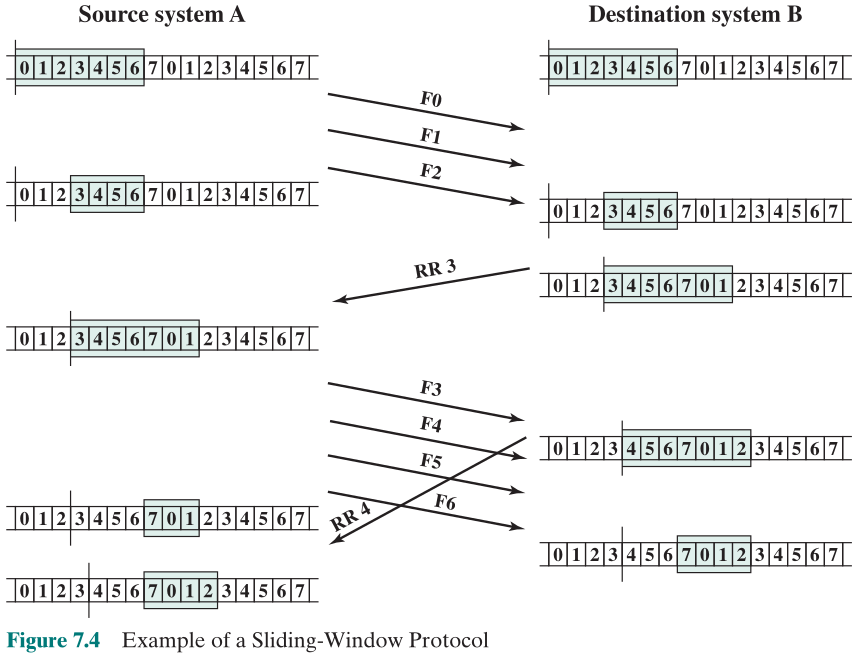
\includegraphics[width=0.8\linewidth]{img/img04}
	\end{center}
\end{frame}

\begin{frame}
	\frametitle{Sliding Window Utilization}
	\begin{itemize}
		\item Window size $ W $, transmission time = 1, propagation time = $ a $
		\item Case 1: $ W >= 2a + 1 $
		\begin{itemize}
			\item Sender A can transmit continuously with no pause and normalized throughput is 1.0
		\end{itemize}
		\item Case 2: $ W < 2a + 1 $
		\begin{itemize}
			\item Sender A exhausts its window at $ t = W $ and cannot send additional frames until $ t = 2a + 1 $.
			\item Normalized throughput is $ W/(2a+1) $
		\end{itemize}
	\end{itemize}
\end{frame}

\begin{frame}
	\frametitle{Error Control Techniques}
	\begin{itemize}
		\item Detection and correction of errors such as:
		\begin{itemize}
			\item Lost frames: a frame fails to arrive at the other side
			\item Damaged frames: frame arrives but some of the bits are in error
		\end{itemize}
		\item Common techniques use:
		\begin{itemize}
			\item Error detection
			\item Positive acknowledgment
			\item Retransmission after timeout
			\item Negative acknowledgement \& retransmission
		\end{itemize}
	\end{itemize}	
\end{frame}

\begin{frame}
	\frametitle{Automatic Repeat Request (ARQ)}
	\begin{itemize}
		\item Collective name for error control mechanisms, including:
		\begin{itemize}
			\item stop and wait
			\item go back N
			\item selective reject (selective retransmission)
		\end{itemize}
		\item Effect of ARQ is to turn an unreliable data link into a reliable one
	\end{itemize}
\end{frame}

\begin{frame}
	\frametitle{Stop and Wait ARQ}
	\begin{itemize}
		\item Source transmits single frame
		\item wait for ACK
		\item if received frame damaged, discard it
		\begin{itemize}
			\item transmitter has \textbf{timeout}
			\item if no ACK within timeout, \textbf{retransmit}
		\end{itemize}
		\item if ACK damaged,transmitter will not recognize it
		\begin{itemize}
			\item transmitter will retransmit
			\item receive gets two copies of frame
			\item use \textbf{alternate numbering} and ACK0 / ACK1
		\end{itemize}
	\end{itemize}
\end{frame}

\begin{frame}{Stop and Wait ARQ}
	\begin{multicols}{2}
		\begin{center}
			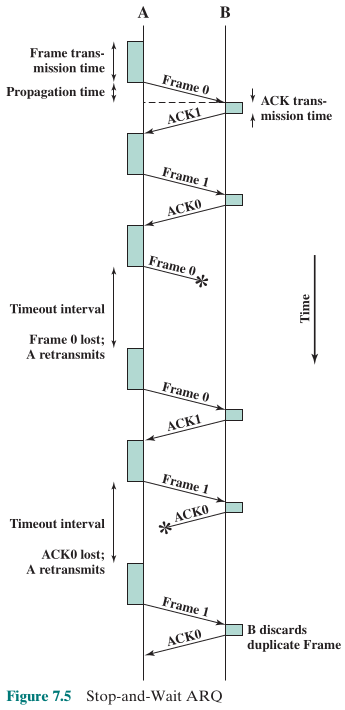
\includegraphics[height=0.9\textheight]{img/img05}
		\end{center}
		\begin{itemize}
			\item see example with both types of errors
			\item pros and cons
			\begin{itemize}
				\item simple
				\item inefficient
			\end{itemize}
		\end{itemize}
		\vfill\null
	\end{multicols}
\end{frame}

\begin{frame}
	\frametitle{Go-Back-N ARQ}
	\begin{itemize}
		\item Most commonly used error control
		\item Based on sliding-window
		\item Use window size to control number of outstanding frames
		\item While no errors occur, the destination will acknowledge incoming frames as usual
		\begin{itemize}
			\item RR=receive ready, or piggybacked acknowledgment
		\end{itemize}
		\item If the destination station detects an error in a frame, it may send a negative acknowledgment
		\begin{itemize}
			\item REJ=reject
			\item Destination will \textbf{discard that frame and all future frames until the frame in error is received correctly}
			\item Transmitter must \textbf{go back and retransmit} that frame and all subsequent frames
		\end{itemize}
	\end{itemize}
\end{frame}

\begin{frame}
	\frametitle{Selective-Reject (ARQ)}
	\begin{itemize}
		\item Also called selective retransmission
		\item Only rejected frames are retransmitted
		\item Subsequent frames are accepted by the receiver and buffered
		\item Minimizes retransmission
		\item Receiver must maintain large enough buffer
		\item More complex logic in transmitter
		\begin{itemize}
			\item Less widely used
		\end{itemize}
		\item Useful for satellite links with long propagation
		delays
	\end{itemize}
\end{frame}

\begin{frame}{Selective-Reject (ARQ)}
	\begin{itemize}
		\item Window Size Limitation
		\begin{itemize}
			\item For a $ k $-bit sequence number, the maximum window size is limited to $ 2k-1 $.
		\end{itemize}
	\end{itemize}
	\begin{center}
		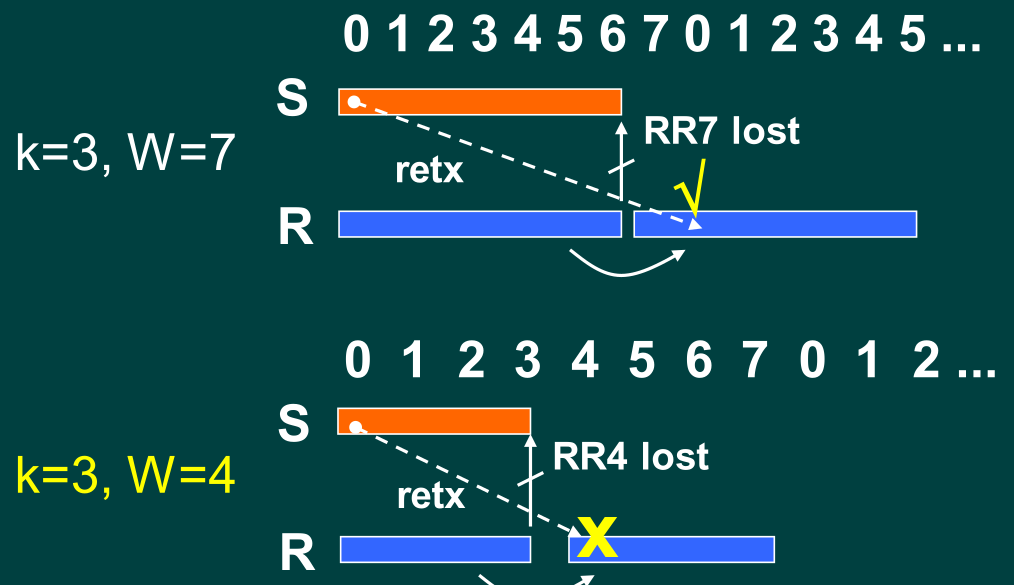
\includegraphics[height=0.6\textheight]{img/img06}
	\end{center}
\end{frame}

\begin{frame}
	\frametitle{Go Back N vs Selective Reject}
	\begin{center}
		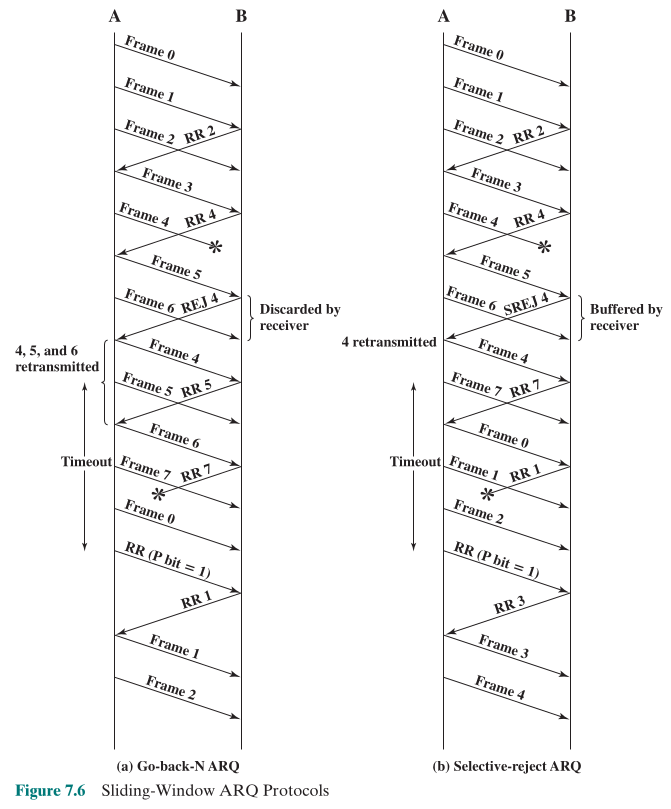
\includegraphics[height=0.9\textheight]{img/img07}
	\end{center}
\end{frame}

\begin{frame}
	\frametitle{High Level Data Link Control (HDLC)}
	\begin{itemize}
		\item An important data link control protocol
		\item specified as ISO 33009, ISO 4335
		\item station types:
		\begin{itemize}
			\item Primary - controls operation of link
			\item Secondary - under control of primary station
			\item \textbf{Combined} - issues commands and responses
		\end{itemize}
		\item link configurations
		\begin{itemize}
			\item Unbalanced - 1 primary, multiple secondary
			\item \textbf{Balanced} - 2 combined stations
		\end{itemize}
	\end{itemize}
\end{frame}

\begin{frame}
	\frametitle{HDLC Transfer Modes}
	\begin{itemize}
		\item Normal Response Mode (NRM)
		\begin{itemize}
			\item Unbalanced config, primary initiates transfer
			\item Used on multi-drop lines, eg host + terminals
		\end{itemize}
		\item \textbf{Asynchronous Balanced Mode (ABM)}
		\begin{itemize}
			\item Balanced config, either station initiates transmission, has no polling overhead, widely used
		\end{itemize}
		\item Asynchronous Response Mode (ARM)
		\begin{itemize}
			\item Unbalanced config, secondary may initiate transmit
			without permission from primary, rarely used
		\end{itemize}
	\end{itemize}
\end{frame}

\begin{frame}
	\frametitle{HDLC Frame Structure}
	\begin{itemize}
		\item synchronous transmission of frames
		\item single frame format used
	\end{itemize}
	\begin{center}
		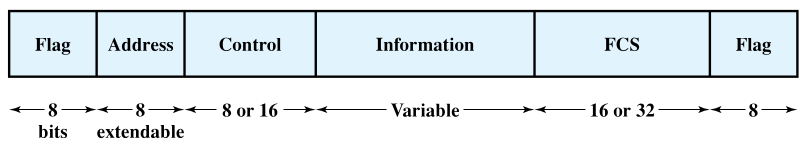
\includegraphics[width=0.8\textwidth]{img/img08}
	\end{center}
\end{frame}

\begin{frame}
	\frametitle{Flag Fields and Bit Stuffing}
	\begin{itemize}
		\item Delimit frame at both ends with 01111110 seq
		\item Receiver hunts for flag sequence to synchronize
		\item Bit stuffing used to avoid confusion with data containing flag seq 01111110
		\begin{itemize}
			\item 0 inserted after every sequence of five 1s
			\item if receiver detects five 1s it checks next bit
			\item if next bit is 0, it is deleted (was stuffed bit)
			\item if next bit is 1 and seventh bit is 0, accept as flag
			\item if sixth and seventh bits 1, sender is indicating abort
		\end{itemize}
		\begin{center}
			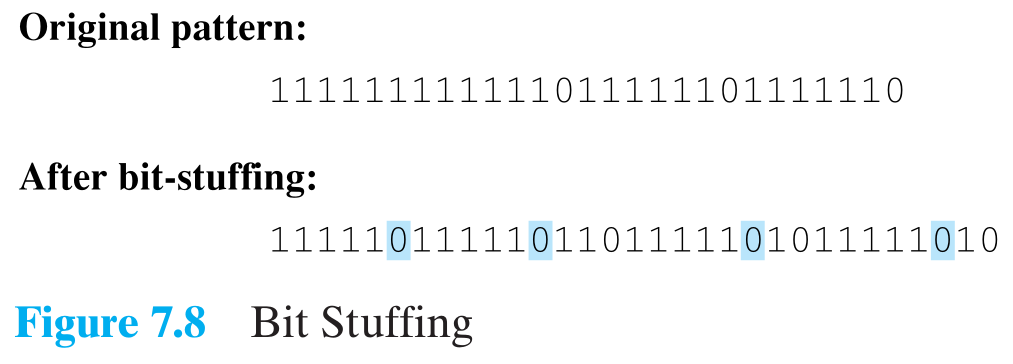
\includegraphics[width=0.7\textwidth]{img/img09}
		\end{center}
	\end{itemize}
\end{frame}

\begin{frame}
	\frametitle{Address Field}
	\begin{itemize}
		\item identifies secondary station that sent or will receive frame
		\item usually 8 bits long
		\item may be extended to multiples of 7 bits
		\begin{itemize}
			\item LSB indicates if is the last octet (1) or not (0)
		\end{itemize}
		\item all ones address 11111111 is broadcast
	\end{itemize}
	\begin{center}
		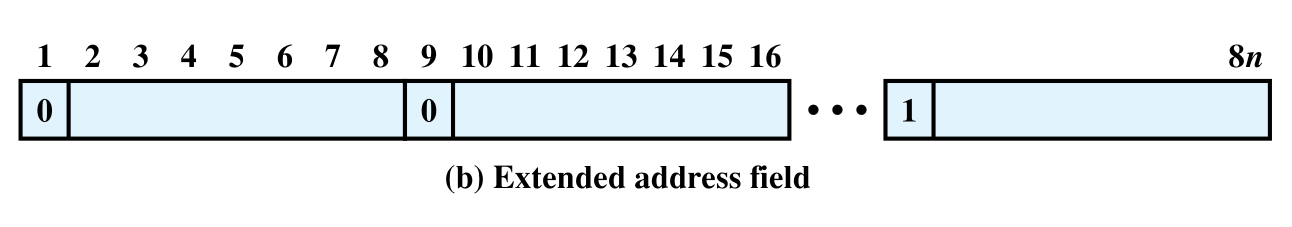
\includegraphics[width=\textwidth]{img/img10}
	\end{center}
\end{frame}

\begin{frame}
	\frametitle{Control Field}
	\begin{itemize}
		\item different for different frame type
		\begin{itemize}
			\item \textbf{Information} - data transmitted to user (next layer up)
			\begin{itemize}
				\item Flow and error control piggybacked on information frames
			\end{itemize}
			\item \textbf{Supervisory} - ARQ when piggyback not used
			\item \textbf{Unnumbered} - supplementary link control
		\end{itemize}
		\item first 1-2 bits of control field identify frame type
	\end{itemize}
	\begin{center}
		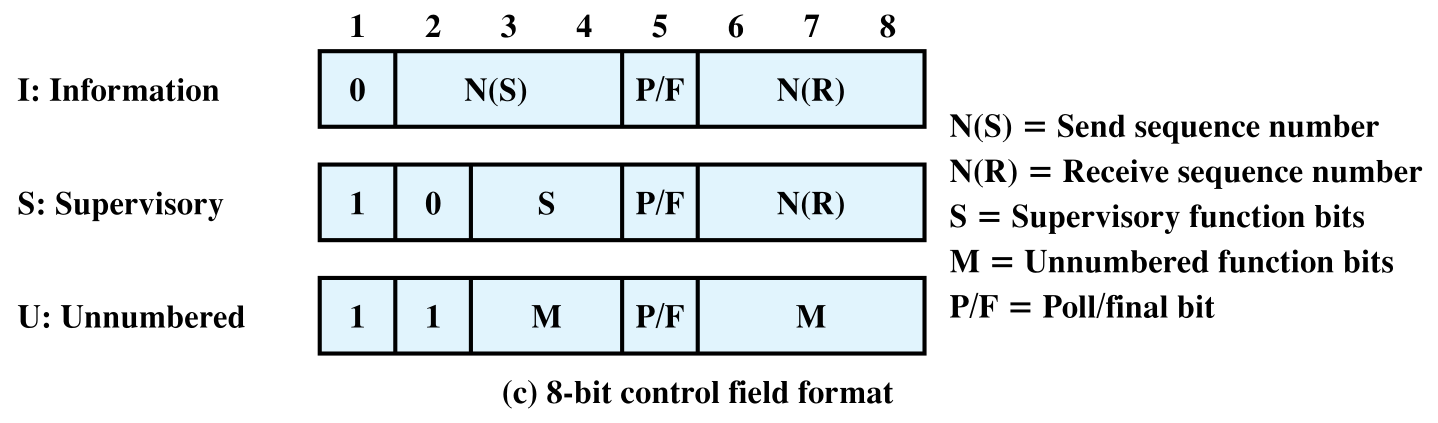
\includegraphics[width=\textwidth]{img/img11}
	\end{center}
\end{frame}

\begin{frame}{Control Field}
	\begin{itemize}
		\item Use of Poll/Final bit depends on context
		\item In command frame is P bit set to1 to solicit (poll) response from peer
		\item In response frame is F bit set to 1 to indicate response to soliciting command
		\item Seq number usually 3 bits
		\begin{itemize}
			\item Can extend to 8 bits as shown below
		\end{itemize}
	\end{itemize}
	\begin{center}
		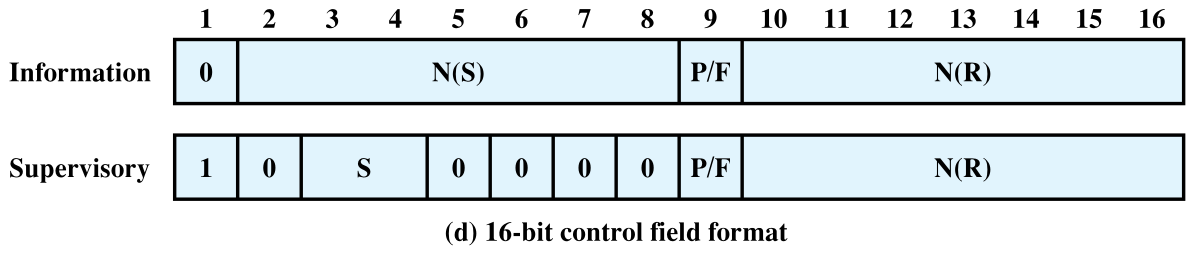
\includegraphics[width=\textwidth]{img/img12}
	\end{center}
\end{frame}

\begin{frame}
	\frametitle{Information and FCS Fields}
	\begin{itemize}
		\item Information Field
		\begin{itemize}
			\item In information and some unnumbered frames
			\item Must contain integral number of octets
			\item Variable length
		\end{itemize}
		\item Frame Check Sequence Field (FCS)
		\begin{itemize}
			\item Used for error detection
			\item Either 16 bit CRC or 32 bit CRC
		\end{itemize}
	\end{itemize}
\end{frame}

\begin{frame}
	\frametitle{HDLC Operation}
	\begin{itemize}
		\item consists of exchange of information, supervisory and unnumbered frames
		\item have three phases
		\begin{itemize}
			\item initialization
			\begin{itemize}
				\item by either side, set mode \& seq
			\end{itemize}
			\item data transfer
			\begin{itemize}
				\item with flow and error control
				\item using both I \& S-frames (RR, RNR, REJ, SREJ)
			\end{itemize}
			\item disconnect
			\begin{itemize}
				\item when requested or fault noted
			\end{itemize}
		\end{itemize}
	\end{itemize}
\end{frame}

\begin{frame}
	\frametitle{HDLC Operation Example}
	\begin{center}
		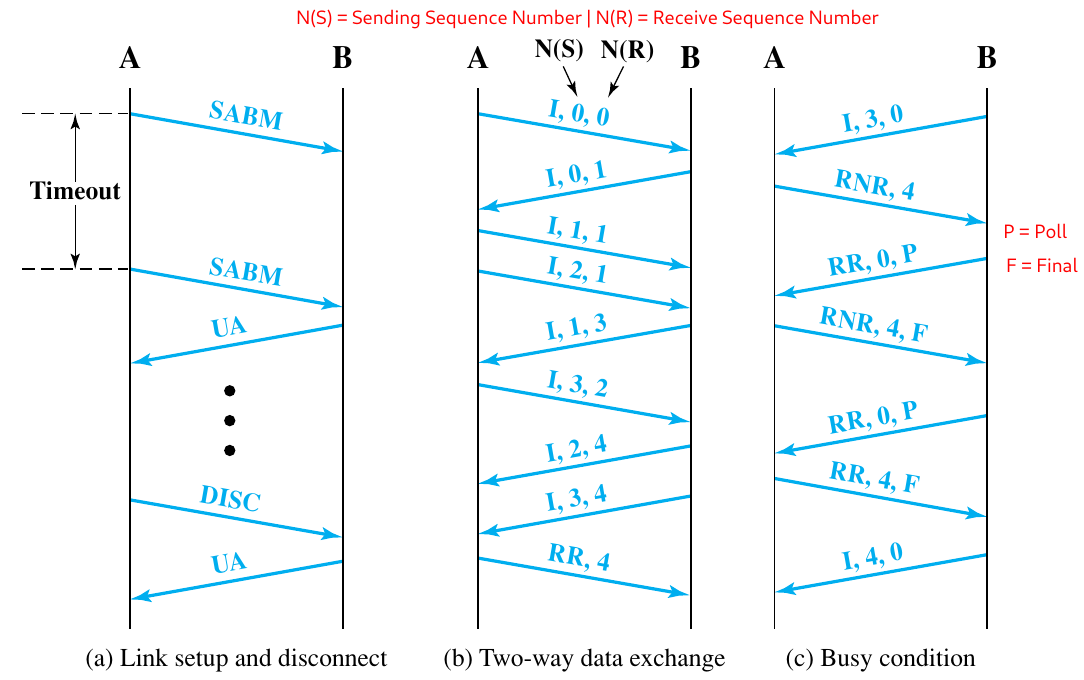
\includegraphics[height=0.8\textheight]{img/img13}
	\end{center}
\end{frame}

\begin{frame}{HDLC Operation Example}
	\begin{center}
		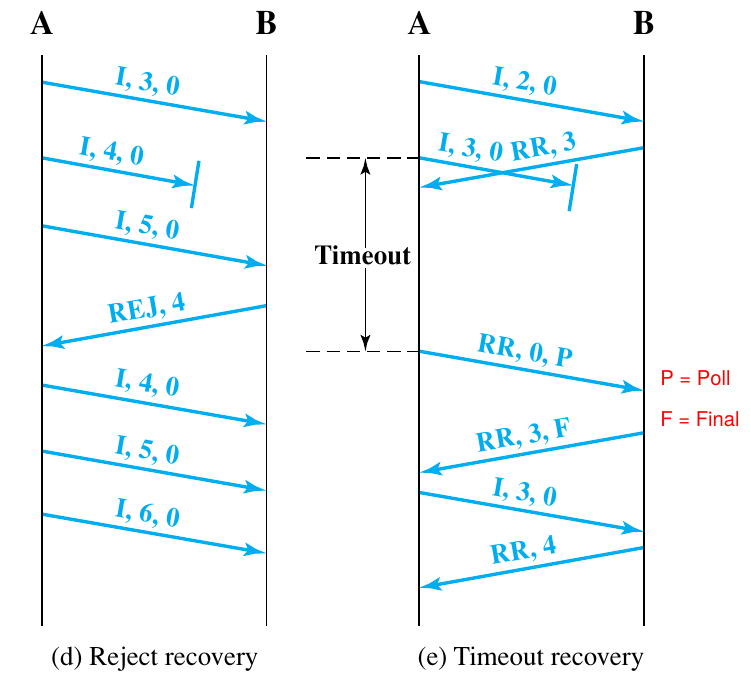
\includegraphics[height=0.8\textheight]{img/img14}
	\end{center}
\end{frame}

\begin{frame}
	\frametitle{Summary}
	\begin{itemize}
		\item Introduced need for
		\item Flow control
		\item Error control
		\item HDLC
	\end{itemize}
\end{frame}

\begin{frame}
	\frametitle{Tugas Mandiri}
	\begin{itemize}
		\item Stallings, W. (2014). Data and Computer Communications, 10th Edition, New Jersey: Upper Saddle River
		\begin{itemize}
			\item Chapter 7 Data Link Control Protocols
		\end{itemize}
		\item Gupta, P. C. (2006). Data Communications and Computer Networks. New Delhi: Prentice Hall of India
		\begin{itemize}
			\item Chapter 5 Error Control
		\end{itemize}
		\item Tanenbaum, A. S. \& Wetherall, D. J. (2013). Computer Networks, Fifth Edition. London: Pearson.
		\begin{itemize}
			\item Chapter 3 The Data Link Layer
		\end{itemize}
	\end{itemize}
\end{frame}

\begin{frame}
	\frametitle{Tugas Terstruktur}
	\textbf{Tampilkan Tugas 6}
\end{frame}

\end{document}
